\chapter{Results}
\label{ch:results}

In the previous chapters we presented an architecture that satisfies the requirements of a VR visualization development workstation. We also presented an implementation of the engine of such an environment that satisfies in particular its performance and generality requirements. To validate our work, we run similar tests to those presented by Dreuning for their OculusVTK environment \cite{dreuning_visual_2016}. We compare the results of these tests with with those from Dreuning and the performances of VtkToUnity \cite{wheeler_virtual_2018}. Finally, we compare those results with the findings from Chapter~\ref{ch:rqrmsandclngs} on the performances of VTK in C++ and Python.

\section{Methodology}

We have developed two Unity scenes using our plugin to test two visualizations using VTK. In Section~\ref{sec:materials} we introduce these scenes. The implementation follows a similar structure to the examples provided by VtkToUnity, but offer less interaction. To each of the VTK objects in the scene, a rotation is applied in order to evaluate the behaviour 

As we are using an HTC Vive headset, we can use the SteamVR provided layer to collect the performance data. Unfortunately, this utility requires us to take these values manually or to record through other software the readings, as there is no way to dump the amount of values we need from this utility. For this reason, we developed a small script in C\# for sampling the FPS values and store them in a buffer that is dumped when the execution of the scene is terminated. We dump at the end of the execution to avoid the IO operations to influence the FPS values. Another script is written to dump profiling values instead. It follows the same structure as the FPS reader, but instead times the execution of the calls to our implementation. 

The scenes are executed manually and navigated through-out the test to evaluate performance over a realistic usage of the environment. The visualization produced are rendered both from afar as well as nearby, through the motion of the user. The visualizations are also scaled using a Unity proxy object that contains the VTK objects, as well as applying a constant spin to the VTK object from within Unity, to account for Unity operations influencing VTK objects. In one scene we also apply repeatedly transformations to the VTK objects using our plugin, in order to take into account real-time changes to the objects.

There should be no graphical artefacts when VTK objects change during runtime and the rendering, scaling and transformation of the objects should not impair usage of the environment. We will finally compare our experience of the environment with the data collected to validate our engine.

The results from these tests should validate in part our performance requirement. Considering we are only instantiating and updating one object at the time, we have to check that the time it takes to execute such operations would not account for major disruption in usage when multiple objects are on screen. We think it to be more interesting to view the profiling data from the scenes over a full test with multiple objects, as we can have a more clear picture of what the limits of the system are.

Nonetheless, we will perform a stress test with an increasing number of objects to complete the discussion. This test will not be run in a VR environment, considering that, if significant differences are found between the two, we can already account for that comparing these results with the previous two.

% Finally, we run some tests with and without adapters for the used objects, in order to take into account the overhead of accessing the introspection layer. These tests will not be run inside a VR environment as they are used as validation for our results from Chapter~\ref{ch:rqrmsandclngs}, and thus it is not important in which environment is run.

We expect our tests to show that the scenes using the introspection layer are indeed slower, heavier or both compared to previous solutions. However, we also expect it to yield a usable environment and as such achieve our objective of developing a powerful enough engine to support general purpose VR visualization development environments. We also expect there to be a significant difference in the execution times compared to the native runs from Chapter~~\ref{ch:rqrmsandclngs}, as we introduce delay both in accessing \acrshort{vtk} and with Unity's rendering cycle. However, seeing as the execution times from the native tests were promising, we expect this not to be an issue.

We also expect our system to be able to support a somewhat large number of simple VTK objects, as the profiling conducted on the C++ with Python introspection shows the operations take times that are insignifcant comapred to the 11.1ms limit we have to reach for the 90 FPS target. If we consider more complex objects such as stream tracers, further optimisations will likely be required for a completely fluid experience with multiple of such objects and live editing, which will be discussed in Chapter~\ref{ch:conclusion}.

\section{Materials}
\label{sec:materials}

To test our design, we implemented the engine of the environment, i.e. the Infrastructure layer and its integration with Unity as described in Chapter~\ref{ch:design}, and developed two test scenes in Unity using the plugin. In order to test them, we used  Python 3.7 to run the scripts and embed the interpreter in a C++11 native plugin. We built the system using CMake 3.14 and MS Visual Studio Community 2015. We tested the implementation with VTK 8.1.2 and 9.0.2 to test its version-agnosticism, and Unity 2019.3.5f1, under Windows 10.

% TODO: add the specifications of the Lab's PC
The environment runs on a workstation built with an Intel(R) Core(TM) i7-7700K CPU @ 4.20GHz, NVIDIA GeForce GTX 1080 Ti and 32.0 GB of RAM. We used a first generation HTC Vive HMD to test the scenes, which has a 90 Hz refresh rate with a combined 2160x1200 pixels. For the tests we used a density dataset file provided by Boston University Tech in a 2008 workshop on Paraview\footnote{Available online at \url{https://www.bu.edu/tech/support/research/training-consulting/presentations/visualizationworkshop08/}.} which we edited in order to have the points centered around (0, 0, 0). 

We track performances using a C\# script in the Unity editor called through a static object loader that collects the FPS count every second and dumps them into a log file. We then process the file in order to produce the following information from the data: the FPS distribution, maximum, minimum, mean and median values. We compare the results with the recommended values from Unity and HTC. During the tests, we move the camera at differening distances from the user and executing delayed updates of the objects in the scene to see how these updates impact the user experience.

The experiments are composed of one scene where a cone is rendered through a \verb|vtkConeSource| and its parameters adjusted so to have a higher resolution. Every two seconds, it's height, radius and resolution are changed. A second scene is composed of a \verb|vtkStreamTracer| generated from the density dataset. We first test the scene using a low number of points for the stream tracer, and then again with a much larger number.

\section{Tests}

We discuss the results of each single test we run. In particular, we focus on analysing the performances and profiling of each of the scenes. For each test we show the relevant pieces of C\# code creating and manipulating the objects. The FPS counter we use for collection is a common piece of code in the Unity community and we will not examine it. The profiling instead is carried out in two different ways. The first, consistent with how the tests in Chapter~\ref{ch:rqrmsandclngs}, computes the time using a timing function on the plugin calls and dumps those to a spreadsheet. The second uses Unity's integrated profiler to generate relevant metrics on the scene's runtime. All the listings shown are stripped of timing and profiling code for readability purposes.

\subsection{Cone Source}

With the Cone source scene, we aim at confirming our environment works well at rendering and manipulating simple objects, while achieving the target performances. The relevant implementation is shown in Appendix~\ref{apx:unity-test-scenes}. This particular scene is also updated every two seconds, changing the cones height, radius and resolution every two seconds. This is done through a coroutine for which the code is shown in Appendix~\ref{apx:unity-test-scenes} The objective is to evaluate the performance of the plugin under realtime editing. Finally, the scene is run both with and without HMD to evaluate how much this influences the plugin's performances.

From our manual tests, the scene appeared well rendered, the updates to the VTK object did not cause lag to the rotation or the rendering of the object, no glitches or artefacts were generated that were not expected, and the experience within the environment felt smooth. The data collected by the scripts further confirms the first-hand experience, as is visible in Figure~\ref{fig:cone-with-updates-analysis}.

In order to understand the graphs, below are the relevant information from the dataset. In particular, the execution of the test lasted for circa 83 seconds. Table~\ref{tab:cone-with-updates-description} relays the rest of the data. As visible, the values validate our design. The system reaches on average and most of the time the objective FPS values, in particular staying stable around 89.0 FPS.

Although this value is not exactly 90 FPS, as would be most desirable, considering the possible rounding error and that these values get dumped as integer values, it is likely that those values approached closely 90 FPS and thus we believe that error accounts for this difference.

What is surprising to see, is the minimum of 2 FPS and quite a large standard deviation. However, we account for such variation considering two main factors. First, we know that our plugin requires a certain loading time to be fully operational, and this loading time is blocking to our scene, as the VTK objects cannot be instantiated yet at this point. Second, we have not cleaned the dataset of potential outliers and thus we may be looking at sharp FPS falls that are not perceivable while using the environment, as proven by the fact that our experience was not disrupted by those drops.

\begin{table}[!t]
    \centering
    \begin{subtable}{.45\linewidth}
        \centering
        \begin{tabulary}{\textwidth}{LR}
            \multicolumn{2}{c}{\textbf{FPS metrics}}       \\ \hline
            Count              & 7405             \\
            Max                & 99               \\
            Min                & 2                \\
            Mean               & 87.7627          \\
            Median             & 89.0             \\
            Standard deviation & 3.1823           \\
            5th percentile     & 88.0             \\
            25th percentile    & 89.0             \\
            50th percentile    & 89.0             \\
            75th percentile    & 89.0            
        \end{tabulary}
        \caption{}
    \end{subtable}
    \begin{subtable}{.45\linewidth}
        \centering
        \begin{tabulary}{\textwidth}{LR}
            \multicolumn{2}{c}{\textbf{FPS metrics processed}}       \\ \hline
            Count              & 7172             \\
            Max                & 92               \\
            Min                & 86               \\
            Mean               & 88.9769          \\
            Median             & 89.0             \\
            Standard deviation & 0.5110           \\
            5th percentile     & 88.0             \\
            25th percentile    & 89.0             \\
            50th percentile    & 89.0             \\
            75th percentile    & 89.0            
        \end{tabulary}
        \caption{}
    \end{subtable}
    \caption{Description of the data distribution of FPS in the cone source scene. (a) does not account for outliers, while (b) does.}
    \label{tab:cone-with-updates-description}
\end{table}

Furthermore, we are collecting metrics and running quite some debugging scripts on top of our plugin, and as such these values could also be explained through all the boilerplate code running. We thus attempt to clean-up the dataset in order to remove these factors, i.e. use the profiling data to remove the loading period from the dataset and we use Z-Scores of threefold the standard deviation to remove outliers from the dataset.

With these considerations, we analyse again the dataset and produce new results that indeed confirm our suspicions and, in fact, validate our design and implementation. We still do not account for the metrics and debugging code, but considering the results we believe those to be trivial and not influencing our results to an interesting degree.

\begin{figure}[t]
    \centering
    \begin{subfigure}{.45\textwidth}
        \centering
        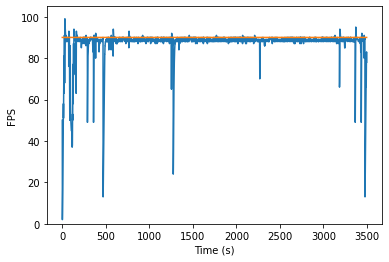
\includegraphics[width=\textwidth]{pictures/analysis cone/output_5_0.png}
        \caption{}
    \end{subfigure}
    \begin{subfigure}{.45\textwidth}
        \centering
        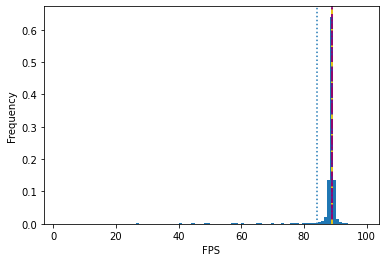
\includegraphics[width=\textwidth]{pictures/analysis cone/output_6_0.png}
        \caption{}
    \end{subfigure}
    \begin{subfigure}{.45\textwidth}
        \centering
        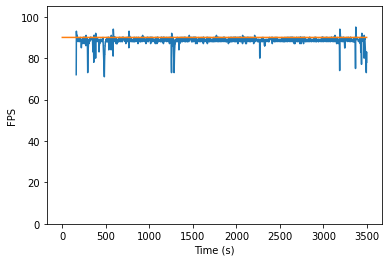
\includegraphics[width=\textwidth]{pictures/analysis cone/output_13_0.png}
        \caption{}
    \end{subfigure}
    \begin{subfigure}{.45\textwidth}
        \centering
        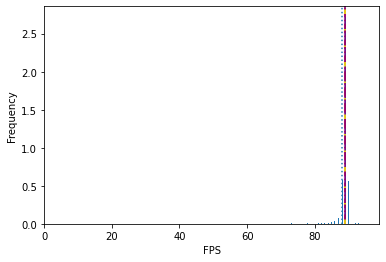
\includegraphics[width=\textwidth]{pictures/analysis cone/output_14_0.png}
        \caption{}
    \end{subfigure}
    \caption{Time series (a), (c) and normal distributions (b), (d) of the FPS from the cone source scene with and wihout outliers respectively. The orange line in (a) and (c) represents the 90 FPS target. The dotted lines in (b) and (d) represent: 5th percentile in blue, 25th in red, 50th in purple and 75th in yellow.}
    \label{fig:cone-with-updates-analysis}
\end{figure}

The amount of time \textit{shaved off} the beginning of the dataset represents the loading time of the software that we do consider for runtime analysis. Furthermore, the missing FPS drops are the outliers in the collected metrics, which amount to 57 frames in total not considered over the 3498 of the entire test (1.63\%). The standard deviation and the mean values also show the app executes as expected under normal load.

We can see both from analysing the profiling data and the FPS that there are some anomalies causing FPS drops and slower operations than expected. The overlapping graphs can be seen in Figure~\ref{fig:overlapping-cone-source-graphs}, where the execution frame of the given value has been computed taking into account each update executes 2 seconds after the previous has terminated (estimated at 180 frames as the error is neglectable). We can see that there is some similarities in the moments when these anomalies where detected, however not enough to hint to an issue with our system.

The remaining values from the profiling are slightly higher than those obtained in Chater~\ref{ch:rqrmsandclngs} for the C++ with Python introspection, but this is as expected and as such validating our results. In particular, it appears it would be acceptable to update a VTK object around 5 to 10 times per frame, which would in total mean between 450 to 900 operations per second. We believe these values could be improved on, but are already an acceptable result.

\begin{figure}[t]
    \centering
    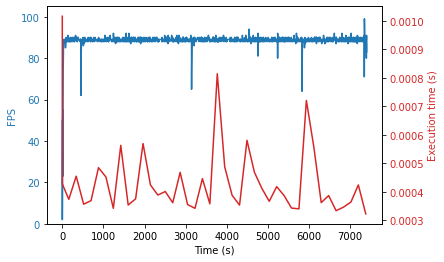
\includegraphics[width=\textwidth]{pictures/analysis cone/output_19_1.png}
    \caption{Overlapping graphs showing the drops in FPS coincide with spikes in computation time of VTK operations.}
    \label{fig:overlapping-cone-source-graphs}
\end{figure}

\subsection{Stream tracer}

The Stream tracer scene has the objective to validate the plugin with more complex sources. The scene has been run both with 100 and 1000 points, and the FPS results analysed as for the cone source scene. The profiling data mainly focuses on update times of the VTK object and their analysis will be discussed later. The relevant implementation is shwon in Appendix~\ref{apx:unity-test-scenes}.

Starting from the 100 points scene, we can clearly see that the system is more than capable to sustain the rendering. The results are fully in line with our expectations and there is not any interesting result to highlight. The description of the dataset are listed in Table~\ref{tab:stream-tracer-100-dataset}, while the time series and distribution can be seen in Figure~\ref{fig:stream-tracer-100-analysis}. Finally, Figure~\ref{fig:stream-tracer-100} shows the rendering inside the VR environment.

Regarding the profiling, the setup operations creating the stream tracer object take around the time we would expect, as they are almost identical to those obtained from the C++ with Python embedding and using introspection test from Chapter~\ref{ch:rqrmsandclngs}. The update operations at each frame were almost neglectable, with a maximum time of 0.15 ms.

\begin{table}[!t]
    \centering
    \begin{subtable}{.45\linewidth}
        \centering
        \begin{tabulary}{\textwidth}{LR}
            \multicolumn{2}{c}{\textbf{FPS metrics}}       \\ \hline
            Count              & 3946             \\
            Max                & 106              \\
            Min                & 2                \\
            Mean               & 88.6607          \\
            Median             & 89.0             \\
            Standard deviation & 4.2957           \\
            5th percentile     & 88.0             \\
            25th percentile    & 89.0             \\
            50th percentile    & 89.0             \\
            75th percentile    & 89.0            
        \end{tabulary}
        \caption{}
    \end{subtable}
    \begin{subtable}{.45\linewidth}
        \centering
        \begin{tabulary}{\textwidth}{LR}
            \multicolumn{2}{c}{\textbf{FPS metrics processed}}       \\ \hline
            Count              & 3716             \\
            Max                & 92               \\
            Min                & 86               \\
            Mean               & 88.9997          \\
            Median             & 89.0             \\
            Standard deviation & 0.5038           \\
            5th percentile     & 88.0             \\
            25th percentile    & 89.0             \\
            50th percentile    & 89.0             \\
            75th percentile    & 89.0            
        \end{tabulary}
        \caption{}
    \end{subtable}
    \caption{Description of the data distribution of FPS in the 100 points stream tracer scene. (a) does not account for outliers, while (b) does.}
    \label{tab:stream-tracer-100-dataset}
\end{table}

\begin{figure}[t]
    \centering
    \begin{subfigure}{.45\textwidth}
        \centering
        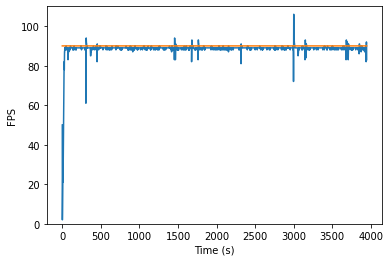
\includegraphics[width=\textwidth]{pictures/analysis stream tracer 100/output_5_0.png}
        \caption{}
    \end{subfigure}
    \begin{subfigure}{.45\textwidth}
        \centering
        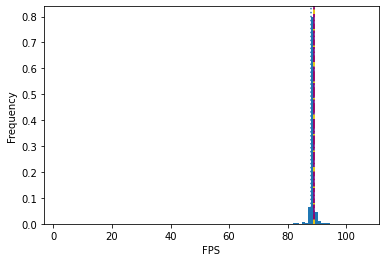
\includegraphics[width=\textwidth]{pictures/analysis stream tracer 100/output_6_0.png}
        \caption{}
    \end{subfigure}
    \begin{subfigure}{.45\textwidth}
        \centering
        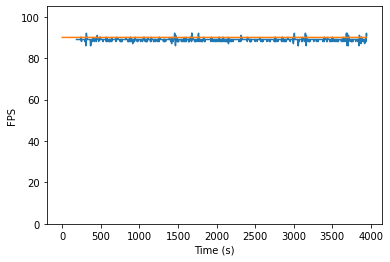
\includegraphics[width=\textwidth]{pictures/analysis stream tracer 100/output_13_0.png}
        \caption{}
    \end{subfigure}
    \begin{subfigure}{.45\textwidth}
        \centering
        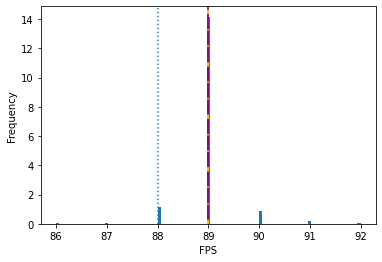
\includegraphics[width=\textwidth]{pictures/analysis stream tracer 100/output_14_0.png}
        \caption{}
    \end{subfigure}
    \caption{Time series (a), (c) and normal distributions (b), (d) of the FPS from the 100 points stream tracer scene with and wihout outliers respectively. The orange line in (a) and (c) represents the 90 FPS target. The dotted lines in (b) and (d) represent: 5th percentile in blue, 25th in red, 50th in purple and 75th in yellow.}
    \label{fig:stream-tracer-100-analysis}
\end{figure}

\begin{figure}
    \centering
    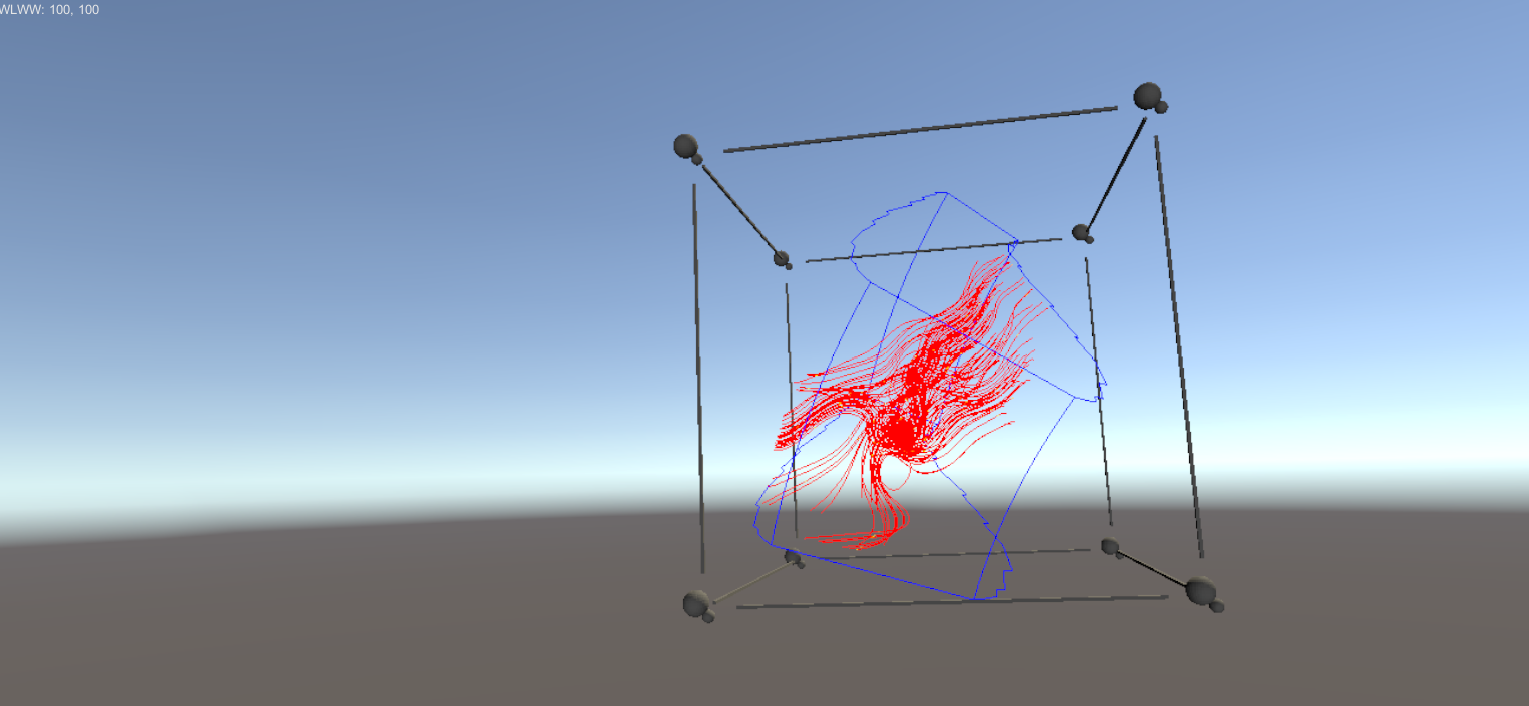
\includegraphics[width=\textwidth]{pictures/stream-tracer-100.png}
    \caption{Image of the stream tracer within the VR environment.}
    \label{fig:stream-tracer-100}
\end{figure}

More interesting is the 1000 points rendering. The distribution of the FPS is more spread out and the standard deviation even without outliers is still significant. Although it reaches hight mean and median values, with solid 90 FPS above the 25th-percentile, the lower end is also more pronounced, with a drop to a minimum of 65 FPS in the processed dataset.

Taking the profiling into account, we can see that the updating operations called on the objects do not take significant amounts of time, with a maximum of just below 0.4 ms. Considering these results, and the weight of the rendering itself, we believe these to be promising results, however they show further work in optimisation is required in order to produce a well rounded system.

The datasets' descriptions are visible in Table~\ref{tab:stream-tracer-1000-dataset}, while Figure~\ref{fig:stream-tracer-1000-analysis} shows the graphs said datasets. Furthermore, Figure~\ref{fig:stream-tracer-1000-profiling} shows the profiling data from this scene. It is important to note two things: first, the first graph does not contain both the update operations called every frame on the stream tracer, neither the first update on the reader object, as its value would make all other values unreadable; second, all the values show that the operations ran by our plugin take considerably little time, and as such we believe most of the lag is caused by optimisations needed at the Unity managed level. The removed values are 0.2771s and 0.2768s for the 100 and 1000 points tests respectively.

As visible from the comparison of profiling data, even though the second scene has a tenfold increase in the amount of points used for generating the stream tracer, times of generation and update are almost identical, evidence of the fact that the system's bottleneck is the Unity managed level and not our engine. We will discuss further root cause investigation in Chapter~\ref{ch:conclusion}.

\begin{table}[!t]
    \centering
    \begin{subtable}{.45\linewidth}
        \centering
        \begin{tabulary}{\textwidth}{LR}
            \multicolumn{2}{c}{\textbf{FPS metrics}}       \\ \hline
            Count              & 8983             \\
            Max                & 101              \\
            Min                & 2                \\
            Mean               & 88.9054          \\
            Median             & 90.0             \\
            Standard deviation & 6.5988           \\
            5th percentile     & 75.0             \\
            25th percentile    & 89.0             \\
            50th percentile    & 90.0             \\
            75th percentile    & 92.0            
        \end{tabulary}
        \caption{}
    \end{subtable}
    \begin{subtable}{.45\linewidth}
        \centering
        \begin{tabulary}{\textwidth}{LR}
            \multicolumn{2}{c}{\textbf{FPS metrics processed}}       \\ \hline
            Count              & 8683             \\
            Max                & 101              \\
            Min                & 72               \\
            Mean               & 89.5098          \\
            Median             & 90.0             \\
            Standard deviation & 4.8100           \\
            5th percentile     & 84.0             \\
            25th percentile    & 89.0             \\
            50th percentile    & 90.0             \\
            75th percentile    & 92.0            
        \end{tabulary}
        \caption{}
    \end{subtable}
    \caption{Description of the data distribution of FPS in the 1000 points stream tracer scene. (a) does not account for outliers, while (b) does.}
    \label{tab:stream-tracer-1000-dataset}
\end{table}

\begin{figure}[t]
    \centering
    \begin{subfigure}{.45\textwidth}
        \centering
        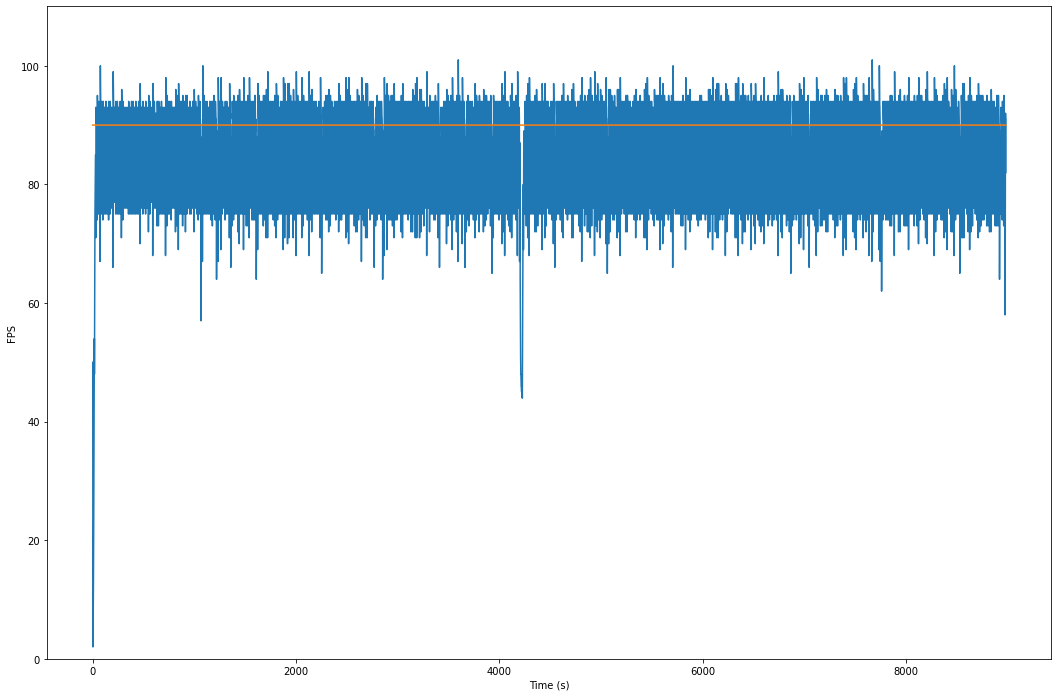
\includegraphics[width=\textwidth]{pictures/analysis stream tracer 1000/output_5_0.png}
        \caption{}
    \end{subfigure}
    \begin{subfigure}{.45\textwidth}
        \centering
        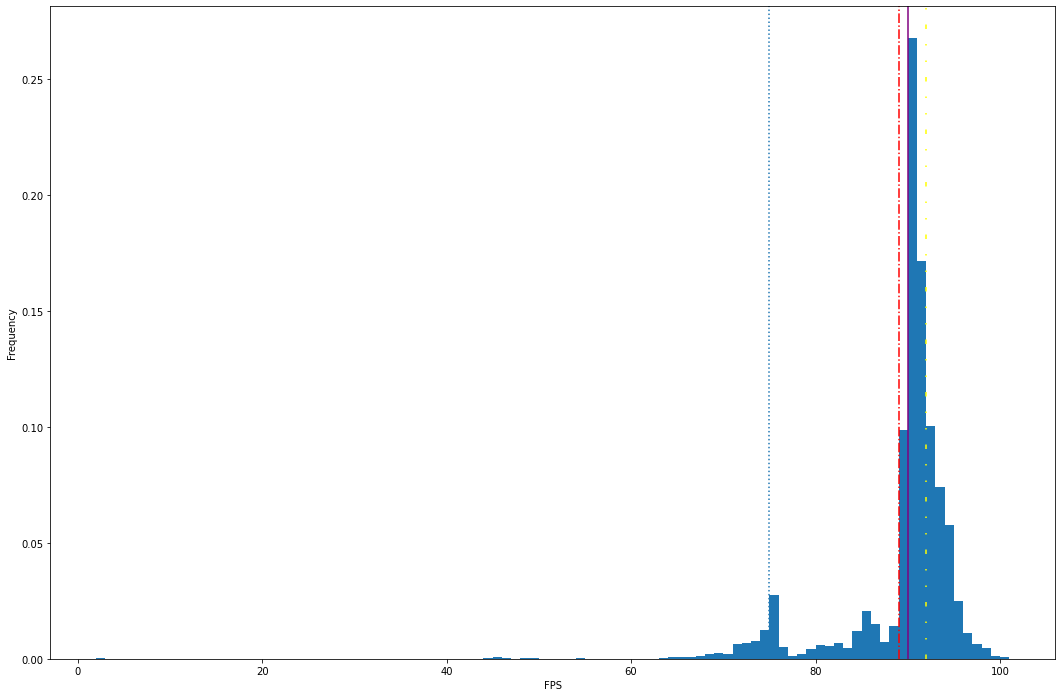
\includegraphics[width=\textwidth]{pictures/analysis stream tracer 1000/output_6_0.png}
        \caption{}
    \end{subfigure}
    \begin{subfigure}{.45\textwidth}
        \centering
        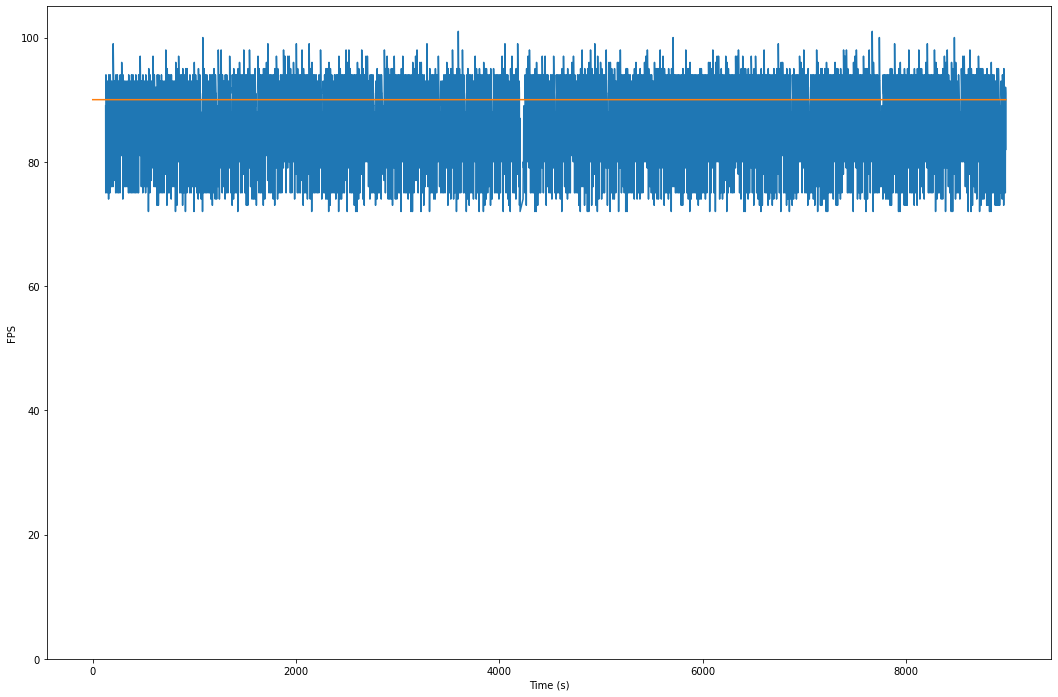
\includegraphics[width=\textwidth]{pictures/analysis stream tracer 1000/output_13_0.png}
        \caption{}
    \end{subfigure}
    \begin{subfigure}{.45\textwidth}
        \centering
        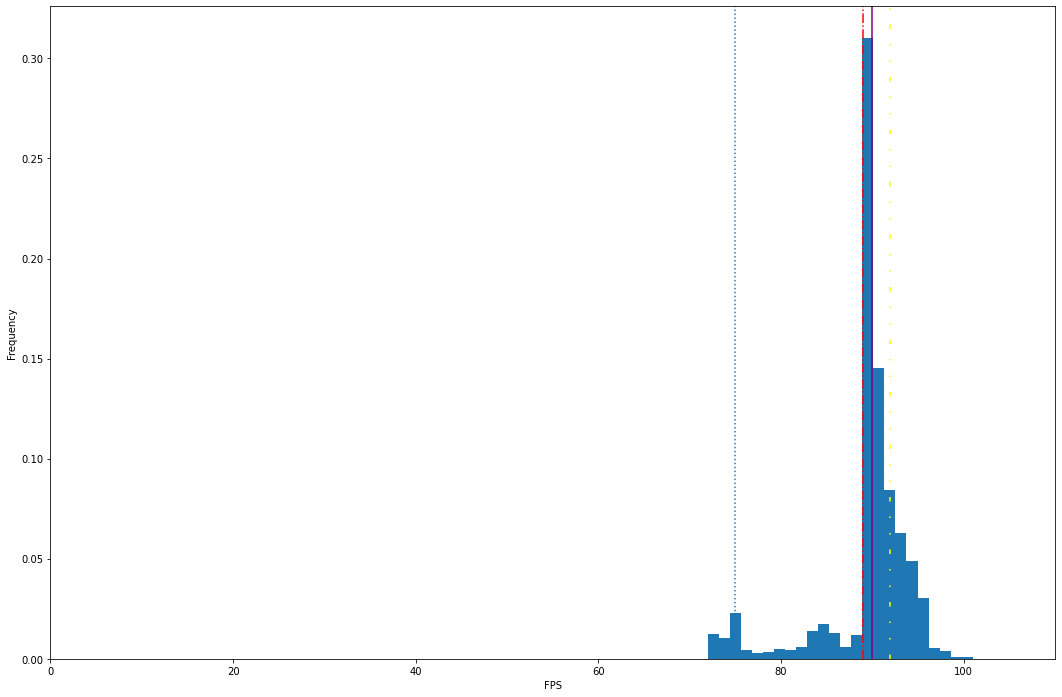
\includegraphics[width=\textwidth]{pictures/analysis stream tracer 1000/output_14_0.png}
        \caption{}
    \end{subfigure}
    \caption{Time series (a), (c) and normal distributions (b), (d) of the FPS from the 1000 points stream tracer scene with and wihout outliers respectively. The orange line in (a) and (c) represents the 90 FPS target. The dotted lines in (b) and (d) represent: 5th percentile in blue, 25th in red, 50th in purple and 75th in yellow.}
    \label{fig:stream-tracer-1000-analysis}
\end{figure}

\begin{figure}
    \centering
    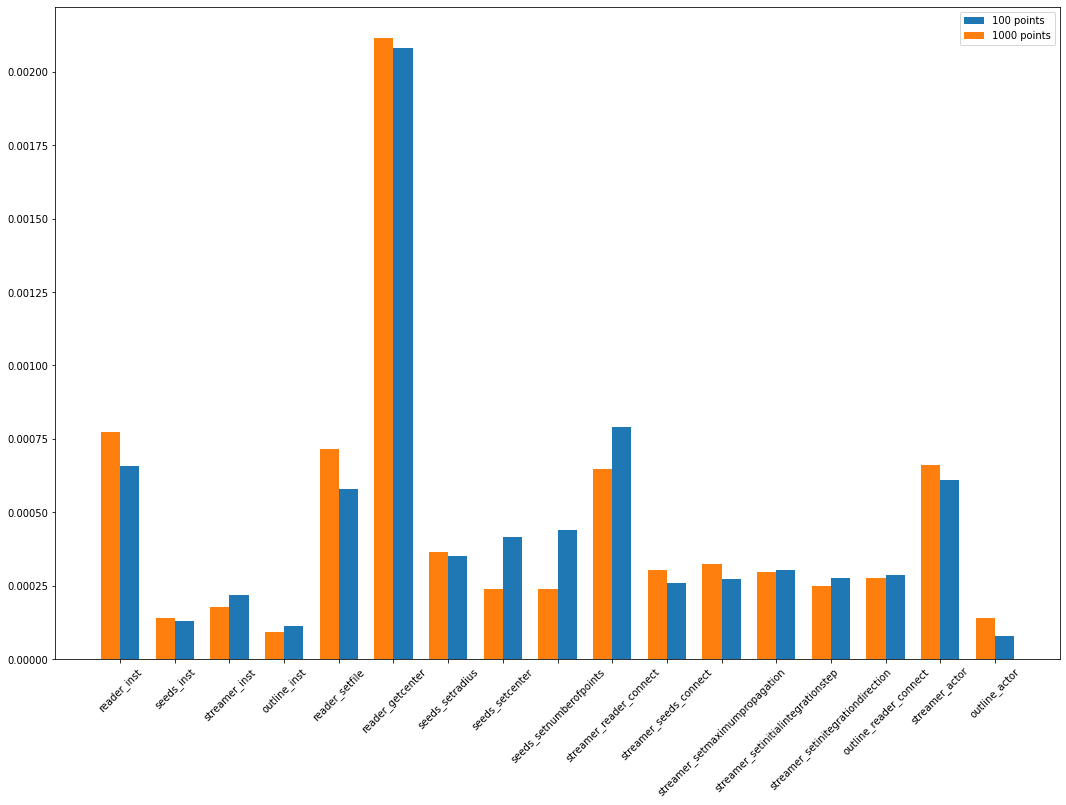
\includegraphics[width=.9\textwidth]{pictures/analysis stream tracer 1000/output_18_1.png}
    \caption{The comparison of time taken by the 100 and 1000 points stream tracers to load.}
    \label{fig:stream-tracer-1000-profiling}
\end{figure}
